\documentclass[a4paper,12pt,abstracton,titlepage]{scrartcl}
\usepackage{fancyhdr}
\usepackage[utf8]{inputenc}
\usepackage[T1]{fontenc}
\usepackage[top=2.5cm, bottom=2.5cm, left=2.5cm, right=2.5cm]{geometry}
\usepackage[affil-it]{authblk}
\usepackage{lipsum}

\author{Maarten Baertsoen, Evergem, Belgium \\
	Daniel S. C. Schiavini, Utrecht, Netherlands\\~}
\affil{Open Universiteit Nederland, faculteit Informatica\\
	T61327 - Afstudeerproject bachelor informatica}
\title{Useful feedback in the\\ Ampersand parser}
\subtitle{Bruikbare feedback in de Ampersand parser \\
	~\\
	Supervisor: Bastiaan Heeren\\
	Examiner: Marko van Eekelen}

\pagestyle{fancy}
\lhead{M. Baertsoen and D.S.C. Schiavini}
\rhead{Useful feedback in the Ampersand parser}
\cfoot{\thepage}
\setlength{\headheight}{15pt}

\publishers{
	\normalfont\normalsize
	\parbox{0.8\linewidth}{
		\textbf{Abstract}. \lipsum[1]
	}
}

\begin{document}
\maketitle
\newpage

\tableofcontents
\clearpage

% !TEX root = ../Parsing.tex
\section{Introduction}
\subsection{Identification}
This document contains the domain \& techniques analysis of the project `Useful feedback in the Ampersand parser'.
The document is the milestone product of the project phase 3a for Daniel S.C. Schiavini, as specified in the project planning \citenac{plan} \citeac{monadic-parsing}.

This document is part of the graduation project of the computer science bachelor at the Open Universiteit Nederland.
The project `Useful feedback in the Ampersand parser' is executed in collaboration with Maarten Baertsoen, with support of the supervisor Dr. Bastiaan Heeren and examiner Prof.dr. Marko C.J.D. van Eekelen.
The assignment is given by Prof.dr. Stef Joosten, who researches how to further automate the design of business processes and information systems by the development of the Ampersand project.

Ampersand is an approach for the use of business rules to define the business processes.
Users describe the business rules in a formal language (ADL), and Ampersand compiles those rules into functional specification, documentation and working software
prototypes.
The main objective of this project is to improve the feedback and maintainability of the Ampersand parser.
See \citenac{plan} for more details on the project.

\subsection{Goals}
The main objective of this phase is to gather information that will support the execution of the project.
This document contains the results of the research on domain and techniques that will support the project group.
It focuses on knowledge acquisition in two interrelated fronts:
\begin{description}
	\item[Haskell parsing libraries]
	In order to build the new Ampersand Parser (or refactor the current one), a research is done to choose the library best suited for the development.
	The appropriate library is chosen based on its design, documentation, features and generated errors.
	
	\item[User-friendly error messages]
	The most important feature of the parser that will be built, is that it should generate user-friendly error messages.
	To understand what kinds of messages can be (and should be) generated, a research will be done on what good errors are and how to generate them.
	This part of the research is done by consulting literature.
\end{description}
%
The results of both subjects culminate in a single section with research conclusions.

\subsection{Document overview}
An introduction is given is this section.
Then, in \autoref{sec:libraries} the choices of user-friendly error messages are elaborated.
In \autoref{sec:errors} the qualities of user-friendly error messages are briefly described, and in \autoref{sec:conclusion} the final conclusion is given.

Finally, in the appendix, a glossary of terms, definitions and abbreviations is given, just as a list of references.

\newpage
% !TEX root = ../Thesis.tex

%requirements plusminus 2 pagina's
\section{Objectives (M-R)}
\label{sec:objectives}
In this section we give an overview of the most important objectives of this graduation project, along with an introduction to the project and its context.
The complete list of objectives as given in the beginning of the project is given in the project planning \citepr{plan}.

\subsection{Ampersand project}
In November 2003, the Business Rules Manifesto \citenac{business-rules} was written, with the main purpose of declaring independence for business rules in the world of requirements.
The manifesto supports the vision of business rules as equivalent to requirements.
This is considered a radical change on how people see the world of business architecture.

In December 2010, Stef Joosten, Lex Wedemeijer and Gerard Michels published the paper `Rule Based Design', presenting the Ampersand approach.
The approach puts the rules in the center, using these rules to define the business processes.
Ampersand is named after the \& symbol with the desire of realizing results for both business and IT, in an efficient and effective way.

In 2011, the Ampersand compiler was created as an open source project.
Since then, the compiler has been improved and applied in both business and academic contexts.
The Ampersand end-users write business rules in a specific language (ADL), and compile that specification into functional specification, documentation and working software prototypes.
\dict{ADL}{Ampersand Design Language}%
These rules are based on agreements between the different stakeholders.

The theory behind Ampersand has been thoroughly studied, and is based on mathe\-matical concepts, e.g. relational algebra and Tarski's axioms.
Using this compiler, users write the requirements in ADL and generate all the system specification independent of the platform.
The main advantage is that the requirement's consistency and traceability are always correct (and even provable), from the lowest level up to the front-end.
The requirements are presented to stakeholders in natural language, guaranteeing that any business expert who knows the context can validate the requirements.
\autoref{fig:generation} depicts the artifacts generated by the Ampersand compiler.
%
\begin{figure}[htb]
	\centering
	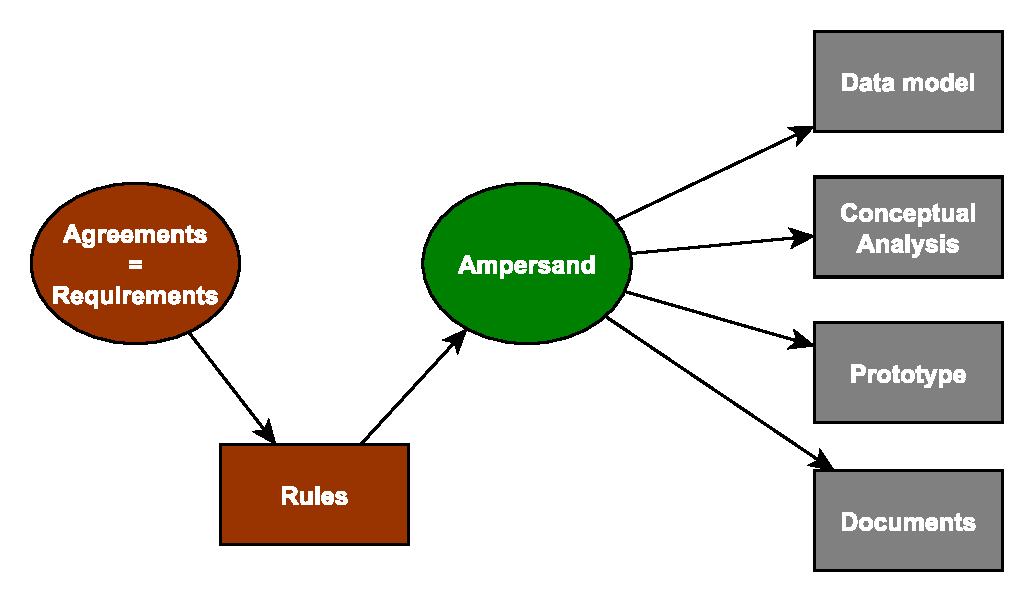
\includegraphics[width=0.7\textwidth]{Figures/Generation}
	\caption[Generated artifacts]{The Ampersand approach generates different artifacts based on the business rules (source: \cite{ampersand-approach})}
	\label{fig:generation}
\end{figure}
%

The Ampersand project is used in several environments, by different user groups.
In a research context, the Ampersand project is part of the research on the use of business rules for software design.
In an academic context, it is also used as the main tool in the course `Ontwerpen met bedrijfsregels' (code T18321) from the Open University of the Netherlands.
Finally, the compiler is used in business environments to design and develop real world business software.

\subsection{High-level architecture}
\label{subsec:architecture}
The compiler developed for the Ampersand research project runs in several steps, hence the Ampersand compiler is also divided in several subcomponents:
\dict{P-structure}{The parse-tree generated by the Ampersand parser, used as input for the type checker}%
\dict{A-structure}{The ADL code generated by the Ampersand type checker, used as input for the calculator component}%
\dict{ADL-structure}{See A-structure}%
\dict{F-structure}{The functional structure generated by the Ampersand calculator, used as input for the different output modules}%
\begin{itemize}
	\item \textbf{Parser}: This component receives the ADL code as input, and parses that code into a parse-tree (also known as P-structure).
	\item \textbf{Type checker}: The Ampersand type checker receives a P-structure as input and converts it into a relational algebra format, suitable for manipulation (also known as A-structure or ADL-structure).
		 The semantics of ampersand are expressed in terms of the A-structure.
	\item \textbf{Calc}: The Calc component receives an A-structure as input, and manipulates it according to the research rules, generating the functional structure (also known as F-structure).
		The F-structure contains all design artifacts needed to write a specification and generate the output.
	\item \textbf{Output components}: All design artifacts present in the F-structure are ready to be rendered.
		Several components use this data structure to generate the wished output.
		The output components currently implemented (and their output formats) are the following: 
		\begin{itemize}
			\item Atlas (HTML interface);
			\item Revert (Haskell source);
			\item Query (prototype generation);
			\item Documentation Generator (Pandoc structure).
		\end{itemize}
\end{itemize}

\subsection{User-friendly parser}
The end-to-end process of the ampersand project, from compiling towards the generated artifacts, is correct, however there is a major improvement topic identified in the first step, the parsing of the input scripts.

One of the main complaints from users is the quality of the errors generated by the Ampersand parser, making it hard for the end users to correct faulty ADL statements.
Since the beginning of the project, the parser subcomponent never received special attention, and it has not been analyzed for improvements.

In order to generate better, useful and to the point error messages, it is assumed that a complete refactoring of the parser will be necessary.
The main challenge is to choose the correct kind of architecture and libraries.
Note that discovering which errors are the most common and what user-friendly messages consist of, is an important part of the assignment.
At the beginning of the project, no list of undesirable error messages is available.
Therefore it was up to us, as a part of the project, to judge which error messages were good enough and which were undesirable.

\subsection{Other objectives}
While designing and implementing the new Ampersand parser, the following objectives were also important:
\begin{itemize}
  \item \textbf{Integration}: The new parser must interface with the remaining Ampersand modules.
    It must thus be implemented in Haskell.
  \item \textbf{Libraries}: Since different implementation options are available, it was important to choose the most suitable Haskell parsing framework.
  \item \textbf{Maintainability}: Well-written and maintainable code is a must for the Ampersand project, since it is an open-source project.
    The maintainability must be either maintained or improved; otherwise the parser is not to be taken into production.
  \item \textbf{Tests}: Testing the parser well was a task for this project.
    The suggestion is to use testing tools to improve the process, e.g. QuickCheck.
  \item \textbf{Pretty-printing}: This is important in order to test the parser.
\dict{HPC}{Haskell Program Coverage}%
\dict{Haddock}{Software documentation generator for the Haskell programming language}%
\dict{HLint}{Statical analysis software that suggests maintainability improvements}%
  \item \textbf{Tools}: Within the Haskell community, several tools are popular to verify code quality and generate documentation, e.g. HPC, Haddock and HLint.
  \item \textbf{Fixed syntax}: The new parser must process the same inputs as the previous parser.
  \item \textbf{Fixed parse tree}: The new parser must produce the same outputs as the previous parser.
    Any further changes must be applied to the rest of the Ampersand system.
\end{itemize}

During the project, some additional requirements have been identified:
\begin{itemize}
  \item \textbf{Git/GitHub}: The changed software had to be integrated into the GitHub Ampersand project.
    The development itself happened in a separate branch of a separate fork, so that deliveries could be merged in a smooth way.
    This was an especially hard requirement for us, since we had no experience with Git.
  \item \textbf{Cabal}: The building system for Haskell had to be maintained as the building platform.
  \item \textbf{EBNF}: The syntax of the Ampersand grammar was specified in EBNF notation but was not up-to-date.
    Any changes to the syntax had to be documented according with this notation.
    One option was to add the EBNF as comment in the source code in order to make clear that the complete grammar is implemented correctly.
\end{itemize}

On top of the project goals, we also wanted to help the university and other students with our results.
Finally, building up knowledge was also important for us (i.e. functional programming, Haskell, compilers, parsers, LaTeX, Ampersand, business rules and research in general).

% !TEX root = ../Thesis.tex

\section{Domain \& techniques}
\label{sec:domain}
% !TEX root = ../Thesis.tex

%algemeen overzicht domeinen en technieken plusminus 2 pagina's
\subsection{Overview}
\label{domain:overview}
Before the actual parser work can start, it is imperative that the project team establishes a solid foundation of the existing system and the environment in which the system is used.
This phase of the project (domains \& techniques) is meant to assure that this knowledge is sufficiently gathered through individual research.
A set of relevant topics needed to support the team during the project execution is listed and allocated to the project team members.
The allocation was based on the aspect that Maarten took the more functional topics where Daniel addressed the more technical topics.
This way, both the domains and the techniques are well covered.

The research of Maarten was focused on the goals of the Ampersand approach as a whole, within the domain of formal specification techniques.
It focuses on the Ampersand vision, the methodology, the way Ampersand is used in practice and the future road-map of the Ampersand approach.
This is depicted in \autoref{domain:approach}.

Daniel investigated the domain of user friendly error messages and how to create them.
The second part of Daniel's research investigated the technical considerations to take into account while selecting a new parser.
Finally, based on the acquired insight, a new parser was selected to be proposed to our project customer.
His research is explained in \autoref{domain:parsing}.

% !TEX root = ../Thesis.tex

% individueel verslag onderzoek deeldomein en bijhorende technieken, plusminus 5 pagina's
% details van domein en technieken in relatie met het onderzoeksproject
% academische verantwoording gemaakte keuzen

\section{The Ampersand approach}
\label{domain:approach}
The research on the Ampersand Approach is done by Maarten Baertsoen.
The objective was to understand the vision of Ampersand in relation towards other formal methods within the same domain.
It focuses on the strengths and weaknesses of formal methods for defining business requirements.
The Ampersand approach is positioned within these formal methods based on the strengths and weaknesses of the different approaches. 

% !TEX root = ../Parsing.tex

\section{The Ampersand Methodology}
\label{sec:AmpersandTheory}

\subsection{Software requirements, the problem statement}

In 1976,  Dr. Thomas E. Bell investigated the domain of requirement engineering \citeac{SoftReqProbs}, sponsored by the Ballistic Missile Advanced Technology Center with the goal to determine the magnitude and characteristics of requirement-related problems in software engineering and to indicate what type of techniques could correct these issues. 
One of the main conclusions was that requirement errors were the most numerous and that these kind of errors are very time-consuming and, hence, costly to correct.
In his conclusion, Dr. Thomas E. Bel advises to use methods and techniques during the requirement engineering process to ensure consistency within and  between the requirements, such as the unique naming of objects and correct relations between the requirements themselves.
Iin addition, he stressed that the applied methods must aid the verification and validation of the requirements.
 
Although the research is ancient history from an IT point of view, the conclusion is actually still very relevant and therefore, methods and techniques to further improve the quality and consistency of the captured requirements are still a hot topic within the domain of requirement engineering.

An important classification of requirements is made by  Prof.dr. Stef Joosten \citeac{Joosten_derivingfunctional} and Prof. dr. Alex Borgida \citeac{JuretaBEM10}, into early phase requirements (the business requirements), and the late phase requirements (the functional specifications). 

\subsubsection{Formal functional specifications}
The initial focus to tackle the requirements issue, in which the research still continuous after 30 years, was on the functional specifications by the introduction of formal methods for functional specifications \citenac{Sommerville10}, which were based on a mathematical representation of the specifications resulting in the ability to analyze, validate and transform them into useful artifacts during the subsequent design and implementation phases. 

As described by  Luqi \& Goguen, J. A. \citeac{LuqiGoguen1997}, these formal methods for functional specifications had a positive impact on the reliability of the software development process, specifically for the purpose of specification analysis, transformation and verification \citeac{Clarke96formalmethods}.
This  reflects  in the elaboration of several mature formal methods.
The formal methods are categorized into two domains:

\dict{Z}{Formal specification notation zed}
\dict{VDM}{Vienna Development Method}
\dict{Larch}{Languages and Tools for Formal Specification}
\dict{LOTOS}{Language Of Temporal Ordering Specification}
\dict{RAISE}{Rigorous Approach to Industrial Software Engineering}

\begin{description}
	\item[Algebraic languages] describing the system in terms of types of data, mathematical operations on those data and their relationships, such as Z \citeac{Spivey89}, VDM \citeac{RISC3820} and Alloy \citeac{Jackson02}.
	\item[Model based languages] using mathematical sets and sequences to express the system specification as a system state model such as OBJ \citenac{Goguen93introducingobj}, Larch \citenac{Guttag93larch:languages} and LOTOS \citeac{BolognesiB87}.
	\item[Hybrid languages] combining features of both algebraic as model-based languages like RAISE \citeac{George03thelogic} and CafeOBJ, an enhancement of the OBJ language \citeac{DiaconescuFO03}.
\end{description}

\subsubsection{Business requirements}
\dict{RML}{Requirement Modeling Language}
Although the positive impact of the formal specification methods, it was recognized that these techniques were not sufficient. Concisely summarized by Prof. dr. Eric S. K. Yu and Prof. dr. John Mylopoulos \citenac{Understandingwhys}, the formal specification methods focus on the `whats' and the `hows' of the desired system without an understanding of the `whys' behind them. 

Within the social environment in which a software system will be introduced, several stakeholders have different goals,  business requirements, and based on these, they will express, often imprecise and inconsistent, expectations. Only by the correct understanding of their business requirements, to a feasible extend, the requirement engineers will truly feel the `whys' needed to derive the correct `whats' and `hows' to support these different goals.

Several early phase requirement modeling languages, RMLs, were introduced and typically included \citeac{JuretaBEM10}: 
\begin{description}
	\item[An ontology of requirements] describing the needed information to capture and the desired properties and behavior of of the to-be system, the view on the world from the perspective of the to-be system. This includes instances such as `Entity', `Activity' and `Assertion' \citenac{RMLRevisited}.
	\item[Modeling primitives,] to model the concepts and the relations within the ontology.
	\item[Methods,] sometimes automated, to verify consistency and to perform additional analysis to verify if the stated requirements will satisfy the business expectations.
\end{description}

\noindent
\dict{CML}{Conceptual Modeling Language}
\dict{Telos }{From the Greek word which means end; the object aimed at in an effort; purpose}
\dict{KAOS}{Knowledge Acquisition in autOmated Specification}
\dict{i*}{i star}
\dict{COTS}{Commercial Off The Shelf}


Early RMLs such as RML\citenac{RMLRevisited}, provided initial methods but suffered from drawbacks such as extensibility as the provided ontologies were rather fixed meaning that no new notions on par with the existing instances could be addressed. CML \citenac{CML} , which evolved to Telos \citeac{mylopoulos90telos}, contained already additional flexibility. 

KAOS \citeac{KAOS} introduced the notion of `stakeholder goal' where i* \citeac{yu97a} even differentiated between independent and interrelated, joint goals.
Further research to introduce the concept of goal priorities is ongoing for which a new abstract requirements modeling language `Techne' \citeac{JuretaBEM10} is designed, based on the CORE ontology for requirements \citenac{JuretaMF08}. Techne will provide the framework for new RMLs containing methods to compare candidate solutions and their compliance towards the business requirements, a feature that will come in handy as many software engineering projects nowadays includes COTS package based solutions.

\subsubsection{Limitations and frequent issues}
\label{sec:drawbacks}
Besides the significant improvements and their positive impact in software engineering projects, several striking drawbacks related to the use of formal methods are identified \citeac{Joosten_derivingfunctional, LuqiGoguen1997}:
\begin{description}
	\item[Communication] Communication between the business users and the requirement engineers based on the mathematical model is difficult as the business users are not used with mathematical notations. Although the functional specifications are analyzed to make sure they are consistent, it still offers no guarantee that the business requirements are consistent and transformed correctly into functional specifications as they cannot be correctly understood by the end users.
	\item[Typical experience and knowledge of developers] Software developers are not used to develop based on mathematical models, or even lack the skills of higher mathematics. It requires extensive training for these developers to understand the mathematical models and to develop efficiently in these kind of software projects.
	\item[Theoretical approaches] Many formal methods are theoretical and their appliance is demonstrated by means of very simplified example, but when they are effectively used in practice, the gap between theoretical specification and practical coding appears to be problematic, not to say impossible.
	\item[Agile development] Building a formal specification of a complete system is sometimes perceived as not flexible towards agile development techniques in which a system is engineered incrementally. 
	\item[Package based development] Many large software projects nowadays are using package based, COTS, solutions which are configured to fit the needs of the users. In such projects this package is mostly kept as standard as possible, meaning that no or little development is added and the functionalities of the package are used as implemented. In most commercial packages, no specific formal information is provided that allow the use of formal verification and validation techniques. The same goes for cloud solutions which are offered as-is without any, or only very limited, room for changes.
	\item[From business requirements towards functional requirements]Early and late phase requirement methods tend to focus on their specific domain, business of functional requirements, not many methods provide a means to verify the translation from business to functional requirements.
	\item[Supporting tools] Most formal methods don't have supporting tools making it very cumbersome to use them in larger scaled projects, even when there are supporting tools available, they often lack a suitable user interfaces due to which the practical use is threatened.

\end{description}


\subsection{The goals of the Ampersand Methodology}
   
The Ampersand Methodology was founded in 2007 by the inventor Prof.dr. Stef Joosten  \citeac{Joosten_derivingfunctional}, with the vision to provide an answer to several of the main drawbacks of using formal techniques  in software engineering (listed in section \autoref{sec:drawbacks}). 
The Ampersand Methodology is  developed to provide a method to unify the informal process of capturing the needs of users with the formal process of specifying an information system and to provide a formal translation method between both processes, including the necessary tools to ensure that the methodology is useful in real life projects.
Special attention is given to the transformation and verification of the business requirements into functional specifications.

Bottom line, the methodology presents the means to structure and present requirements in such a way that they can be validated by end-users as well as be interpreted unambiguously by system engineers after an automated transformation into functional specifications and design artifacts while the consistency between both is guaranteed.

The Ampersand Methodology addresses several goals to achieve this vision:
\begin{description}
	\item[Communication]  To assure that the stakeholders can correctly understand and validate their needs, the requirements must be documented in a natural language to enable them, without any requirement engineering knowledge, to validate the formal system requirements. On the other hand, the requirements must be structured into formal  functional specifications to make them useful during the actual software development phase and to benefit from the advantages of formal methods. 
	\item[Completeness]A software system in which not all requirements are supported is useless. The Ampersand language must be fully declarative, meaning that all the requirements must be supported in the method to assure that all business requirements, relevant to the subsequent software system, are accommodated correctly in the system specification.
	\item[Consistency]One of the main goals of the Ampersand Methodology is to guarantee consistency, each specified requirement must be applicable, and respected, to all processes in the context of this requirement. The methodology needs to provide the means to assure this consistency.
	\item[Traceability] The requirements must be traceable in such a way that end-users can trace  functions back to the stated business requirements, allowing them to fully understand to reason why these functions are defined.
	\item[Supporting tools] In order to facilitate the adoption of the Ampersand Methodology outside an academic environment, Prof.dr. Stef Joosten defined the additional goal that the Ampersand Methodology must be accompanied with supporting tools to support the requirement engineers and this by creating design artifacts to be used by the software developers.
\end{description}

\subsection{The Ampersand approach}
The Ampersand Methodology introduces a specific approach how to achieve the specified goals. The Ampersand Methodology can support different languages, a specific instance called `Ampersand Definition Language', ADL, is implemented to support the Ampersand Methodology.
The reasoning used to explain the achievement of the different goals is based on ADL.

\subsubsection{Communication}

One of the key differentiators of this approach is that the business requirements are presented towards the stakeholder in natural language while the system engineers can use functional specifications which are automatically transformed from the business requirements, assuring the functional specification is consistent with the business requirements.

The innovative aspect of the Ampersand methodology to achieve this goal is that the business requirements are  represented as `business rules' using relational algebra. A business rule must be seen as a business requirement in the form of an invariant to be satisfied by the business. The business rules are transformed in an automated way by an accompanying ADL tool, assuring the correctness of the functional specification based on the relational algebra of the business rules. Once the functional specifications are generated, the ADL tool will transform them back into the business rules for business user validation. When the re-translated requirements are then still correct for the end users, the system engineers have the assurance that the functional specifications are fully consistent with the business requirements. 

The use of natural language is further facilitated by the fact that it is not limited to a single specific language, it supports any language that satisfies a predefined set of axioms that can be used, making it possible to address each business user in his own language.

\subsubsection{Completeness}
Initial methodologies to define business requirements lacked the power to add new notions besides the pre-defined instances. ADL is designed as a purely declarative language to avoid this drawback. ADL features user specified rules, in relational algebra, design patterns, defined as sets of rules, contexts in which rules are applied and a signaling construct. In ADL, rules are specified without specific pre-defined actions to avoid that they become too narrow, compromising the declarative aspect of ADL.

\subsubsection{Consistency}
Expressing each business requirement as a business rule using relational algebra provides a mathematical foundation to check all rules against each other and to identify inconsistency between two or more business rules.  Checking each rule on his consistency towards the full set of defined business rules manually is quite demanding and would compromise the efficiency of the method on real life projects. 
The consistency check is therefore automated by the supporting tool.

\subsubsection{Traceability}
Business requirements have a one-to-one relationship with business rules offering traceability back from a specific rule, specification, to the business requirement making it possible for the end-user to correctly identify the reasons why the business rule was identified.

\subsubsection{Supporting tools}
The practical use of the Ampersand Approach is supported by a tool built in the functional programming language Haskell. 
This tool produces a wide range of functionalities and design artifacts to support the validation, consistency checks and the subsequent software development steps:
\begin{description}
	\item[Business rules and consistency issues] The inputted business rules in ADL are compiled and typed checked.
	This is realized by using the Swierstra's combinator package for the compiler \citeac{uu-doc}  and the AG-preprocessor by Dijkstra and Swiestra for the type-checker \citenac{MiddelkoopDS10}.
	\item[Data model]  Class diagrams and entity-relationships are created using the the GraphViz package \citenac{gansner2006drawing}. 
	\item[Service catalogue] All possible services on the defined classes and relationships, such as create, get, update and delete,  are specified formally. This formal representation together with the pre- and postconditions of the service make it possible that several developers can program the services independently of each other. 
	It is up to the requirement engineers to determine which services that need to be implemented.
	\item[Function point analysis] A function point analysis providing an insight on the complexity of the system to be built  is generated according to the IFPUG guidelines (\url{http://www.ifpug.org/}). This degree of complexity can be used to estimate the remaining system development effort taking into account the impact of the Ampersand tool as an accelerator
	\item[Software prototype] A remarkable aspect of the Ampersand tool is that it makes it possible to generate a working prototype. The prototype is generated as a web application and uses a MySQL database.
\end{description}
 
\subsubsection{Training}
Although the Ampersand Methodology, including ADL, is not yet widely adopted in the domain of requirement engineering, the methodology, including the supporting tools, is educated by the Open University of the Netherlands, course `Ontwerpen met bedrijfsregels'. A specific site is dedicated to the methodology, as well for self-tuition or co-development purposes.

\noindent




% !TEX root = ../Parsing.tex

\section{User-friendly error messages}
\label{sec:errors}

\subsection{Parsing errors}
When a parser is executed and is unable to recognize the input text, an error is raised.
The main problem when this happens, is that the parser cannot know for sure what the programmer meant to write.
Only the programmer can know exactly what the purpose of the invalid input was.

However, parsers should be able to recognize the most common errors, and support the user to correct them.
Spenke et al. \cite{error-recovery} discuss the following assumptions regarding parsing errors:
\begin{enumerate}
	\item An incorrect program is very similar to a correct one;
	\item An error is very soon followed by a correct piece of program;
	\item There are symbols (e.g. keywords) that are ommited quite rarely, while some less important symbols are more frequently ommited (e.g. semicolons);
	\item There are some very reliable symbols which most likely do not occur by accident, but always in an specific context (e.g. then being part of an if statement);
	\item  If an error cannot be corrected by deletion and/or insertion of a few symbols, the reason is often a complete, misplaced syntactic unit, such as a whole expression where only a single constant is allowed;
	\item A frequent reason for syntax errors is typing errors. In addition, similar basic symbols, such as round and square brackets may easily be confused.
\end{enumerate}

\subsection{User-friendliness}
There is no formal definition of what user-friendly error messages are.
Indeed, an expert programmer will expect to see more details than an unexperienced student.

Therefore, it may be very important to be able to finetune the errors shown.
The developers of the compiler may want details of the inner workings of the system (e.g. the parse tree).
Students, on the other hand, may just want to see the most likely cause of their mistake.

\subsection{Implications for the Ampersand parser}
\label{subsec:errors-ampersand}
The following items have been identified in the literature as important in the error messages generated by parsers:
\begin{description}
	\item[Location] When an error is detected, it is crucial to point out where in the input text the error has been found.
		If the location is incorrect, the user will have to search through his/her entire program to find the syntax error \cite{helium-parser,uu-doc,error-correcting,parsec}.
	\item[Production rules] Listing which product rules are applicable at that moment can help the user to choose the correct one \cite{helium-parser}.
		However, students have been reported to get overwhelmed by the huge list of terminals currently generated by Ampersand in the case of errors \cite{heeren-error}. 
	\item[Misspellings] Very often, errors happen because the users mistype keywords and/or symbols.
		Tokens that are invalid, but very close to valid input and often misspelled, should be recognized by the parser \cite{helium-parser,error-recovery}.
	\item[Error recovery] When an error occurs, it is appropriate that the parser is able to recover from that error.
		This way, the parser can continue analyzing the input \cite{error-correcting,error-recovery}.
\end{description}

% !TEX root = ../ResearchContext.tex

\section{Conclusion}
\label{sec:conclusion}
The Ampersand approach is situated within several research contexts, such as the Business Rule Approach and formal systems.
Additionally, the Ampersand Parser is part of a broader parser research context.
Our conclusion is that the new Ampersand parser has a very small influence in its research context for business rules.
This parser does not offer any new features or improvements to the language.
The largest influence of the project is commercial and educational by improving the user experience.
We expect that the new parser will allow commercial, research and educational users to do their work faster and more efficiently.



% !TEX root = ../Thesis.tex

% individueel verslag onderzoek deeldomein en bijhorende technieken, plusminus 5 pagina's
% details van domein en technieken in relatie met het onderzoeksproject
% academische verantwoording gemaakte keuzen

\subsection{Parsing Libraries \& Friendly Errors}
\label{domain:parsing}
The research on parsing library and user-friendly error messages was done by Daniel Schiavini.
The objective was to gather enough technical information to support the design and implementation of the new Ampersand parser.
It focuses on knowledge acquisition in two interrelated fronts: a search for the parsing library best suited for this project and defining what constitutes good error messages.

The first choice made was to use a combinator library, instead of a parser generator.
The main reason to avoid parser generators is that it is hard to generate useful feedback.
It was then made clear that besides generating good messages, those messages should also be customizable.
Considering the library design, documentation, features, generated errors and error customization, Parsec was judged to be the best suited library for the new parser.
This advice to use Parsec was accepted by the customer.

A list of important consideration points on developing good feedback has been collected through the literature.
Finally, other factors besides error messages are also very important for giving useful feedback.
One of the most important factors is that the documentation should be always kept available, up-to-date, clear and concise.

The complete research report is available as a separate document \citepr{parsing}.

% !TEX root = ../Thesis.tex

%beschrijving van het opgeleverde eindproduct, plusminus 15 pagina’s

\section{Results}
beschrijving van het projectresultaat (het softwaresysteem)
overzicht van de oplossing, met enkele globale voorbeelden

% !TEX root = ../Thesis.tex

\section{Assessment}
\label{sec:assessment}
In this section, we look backwards and explain why some decisions were taken.
In \ref{subsec:assessment-process} we show that we believe the new parser is an adequate improvement to Ampersand.
Then, in \ref{subsec:assessment-approach} we focus on the approach, roles and collaboration within the team.
Finally, in the sections \ref{subsec:assessment-daniel} and \ref{subsec:assessment-maarten}, each of the project members go shortly into their experiences en learning moments.

\input{Assessment/Process}
% !TEX root = ../Thesis.tex

% individueel verslag onderzoek deeldomein en bijhorende technieken, plusminus 5 pagina's
% details van domein en technieken in relatie met het onderzoeksproject
% academische verantwoording gemaakte keuzen

\section{The Ampersand approach}
\label{domain:approach}
The research on the Ampersand Approach is done by Maarten Baertsoen.
The objective was to understand the vision of Ampersand in relation towards other formal methods within the same domain.
It focuses on the strengths and weaknesses of formal methods for defining business requirements.
The Ampersand approach is positioned within these formal methods based on the strengths and weaknesses of the different approaches. 

% !TEX root = ../Parsing.tex

\section{The Ampersand Methodology}
\label{sec:AmpersandTheory}

\subsection{Software requirements, the problem statement}

In 1976,  Dr. Thomas E. Bell investigated the domain of requirement engineering \citeac{SoftReqProbs}, sponsored by the Ballistic Missile Advanced Technology Center with the goal to determine the magnitude and characteristics of requirement-related problems in software engineering and to indicate what type of techniques could correct these issues. 
One of the main conclusions was that requirement errors were the most numerous and that these kind of errors are very time-consuming and, hence, costly to correct.
In his conclusion, Dr. Thomas E. Bel advises to use methods and techniques during the requirement engineering process to ensure consistency within and  between the requirements, such as the unique naming of objects and correct relations between the requirements themselves.
Iin addition, he stressed that the applied methods must aid the verification and validation of the requirements.
 
Although the research is ancient history from an IT point of view, the conclusion is actually still very relevant and therefore, methods and techniques to further improve the quality and consistency of the captured requirements are still a hot topic within the domain of requirement engineering.

An important classification of requirements is made by  Prof.dr. Stef Joosten \citeac{Joosten_derivingfunctional} and Prof. dr. Alex Borgida \citeac{JuretaBEM10}, into early phase requirements (the business requirements), and the late phase requirements (the functional specifications). 

\subsubsection{Formal functional specifications}
The initial focus to tackle the requirements issue, in which the research still continuous after 30 years, was on the functional specifications by the introduction of formal methods for functional specifications \citenac{Sommerville10}, which were based on a mathematical representation of the specifications resulting in the ability to analyze, validate and transform them into useful artifacts during the subsequent design and implementation phases. 

As described by  Luqi \& Goguen, J. A. \citeac{LuqiGoguen1997}, these formal methods for functional specifications had a positive impact on the reliability of the software development process, specifically for the purpose of specification analysis, transformation and verification \citeac{Clarke96formalmethods}.
This  reflects  in the elaboration of several mature formal methods.
The formal methods are categorized into two domains:

\dict{Z}{Formal specification notation zed}
\dict{VDM}{Vienna Development Method}
\dict{Larch}{Languages and Tools for Formal Specification}
\dict{LOTOS}{Language Of Temporal Ordering Specification}
\dict{RAISE}{Rigorous Approach to Industrial Software Engineering}

\begin{description}
	\item[Algebraic languages] describing the system in terms of types of data, mathematical operations on those data and their relationships, such as Z \citeac{Spivey89}, VDM \citeac{RISC3820} and Alloy \citeac{Jackson02}.
	\item[Model based languages] using mathematical sets and sequences to express the system specification as a system state model such as OBJ \citenac{Goguen93introducingobj}, Larch \citenac{Guttag93larch:languages} and LOTOS \citeac{BolognesiB87}.
	\item[Hybrid languages] combining features of both algebraic as model-based languages like RAISE \citeac{George03thelogic} and CafeOBJ, an enhancement of the OBJ language \citeac{DiaconescuFO03}.
\end{description}

\subsubsection{Business requirements}
\dict{RML}{Requirement Modeling Language}
Although the positive impact of the formal specification methods, it was recognized that these techniques were not sufficient. Concisely summarized by Prof. dr. Eric S. K. Yu and Prof. dr. John Mylopoulos \citenac{Understandingwhys}, the formal specification methods focus on the `whats' and the `hows' of the desired system without an understanding of the `whys' behind them. 

Within the social environment in which a software system will be introduced, several stakeholders have different goals,  business requirements, and based on these, they will express, often imprecise and inconsistent, expectations. Only by the correct understanding of their business requirements, to a feasible extend, the requirement engineers will truly feel the `whys' needed to derive the correct `whats' and `hows' to support these different goals.

Several early phase requirement modeling languages, RMLs, were introduced and typically included \citeac{JuretaBEM10}: 
\begin{description}
	\item[An ontology of requirements] describing the needed information to capture and the desired properties and behavior of of the to-be system, the view on the world from the perspective of the to-be system. This includes instances such as `Entity', `Activity' and `Assertion' \citenac{RMLRevisited}.
	\item[Modeling primitives,] to model the concepts and the relations within the ontology.
	\item[Methods,] sometimes automated, to verify consistency and to perform additional analysis to verify if the stated requirements will satisfy the business expectations.
\end{description}

\noindent
\dict{CML}{Conceptual Modeling Language}
\dict{Telos }{From the Greek word which means end; the object aimed at in an effort; purpose}
\dict{KAOS}{Knowledge Acquisition in autOmated Specification}
\dict{i*}{i star}
\dict{COTS}{Commercial Off The Shelf}


Early RMLs such as RML\citenac{RMLRevisited}, provided initial methods but suffered from drawbacks such as extensibility as the provided ontologies were rather fixed meaning that no new notions on par with the existing instances could be addressed. CML \citenac{CML} , which evolved to Telos \citeac{mylopoulos90telos}, contained already additional flexibility. 

KAOS \citeac{KAOS} introduced the notion of `stakeholder goal' where i* \citeac{yu97a} even differentiated between independent and interrelated, joint goals.
Further research to introduce the concept of goal priorities is ongoing for which a new abstract requirements modeling language `Techne' \citeac{JuretaBEM10} is designed, based on the CORE ontology for requirements \citenac{JuretaMF08}. Techne will provide the framework for new RMLs containing methods to compare candidate solutions and their compliance towards the business requirements, a feature that will come in handy as many software engineering projects nowadays includes COTS package based solutions.

\subsubsection{Limitations and frequent issues}
\label{sec:drawbacks}
Besides the significant improvements and their positive impact in software engineering projects, several striking drawbacks related to the use of formal methods are identified \citeac{Joosten_derivingfunctional, LuqiGoguen1997}:
\begin{description}
	\item[Communication] Communication between the business users and the requirement engineers based on the mathematical model is difficult as the business users are not used with mathematical notations. Although the functional specifications are analyzed to make sure they are consistent, it still offers no guarantee that the business requirements are consistent and transformed correctly into functional specifications as they cannot be correctly understood by the end users.
	\item[Typical experience and knowledge of developers] Software developers are not used to develop based on mathematical models, or even lack the skills of higher mathematics. It requires extensive training for these developers to understand the mathematical models and to develop efficiently in these kind of software projects.
	\item[Theoretical approaches] Many formal methods are theoretical and their appliance is demonstrated by means of very simplified example, but when they are effectively used in practice, the gap between theoretical specification and practical coding appears to be problematic, not to say impossible.
	\item[Agile development] Building a formal specification of a complete system is sometimes perceived as not flexible towards agile development techniques in which a system is engineered incrementally. 
	\item[Package based development] Many large software projects nowadays are using package based, COTS, solutions which are configured to fit the needs of the users. In such projects this package is mostly kept as standard as possible, meaning that no or little development is added and the functionalities of the package are used as implemented. In most commercial packages, no specific formal information is provided that allow the use of formal verification and validation techniques. The same goes for cloud solutions which are offered as-is without any, or only very limited, room for changes.
	\item[From business requirements towards functional requirements]Early and late phase requirement methods tend to focus on their specific domain, business of functional requirements, not many methods provide a means to verify the translation from business to functional requirements.
	\item[Supporting tools] Most formal methods don't have supporting tools making it very cumbersome to use them in larger scaled projects, even when there are supporting tools available, they often lack a suitable user interfaces due to which the practical use is threatened.

\end{description}


\subsection{The goals of the Ampersand Methodology}
   
The Ampersand Methodology was founded in 2007 by the inventor Prof.dr. Stef Joosten  \citeac{Joosten_derivingfunctional}, with the vision to provide an answer to several of the main drawbacks of using formal techniques  in software engineering (listed in section \autoref{sec:drawbacks}). 
The Ampersand Methodology is  developed to provide a method to unify the informal process of capturing the needs of users with the formal process of specifying an information system and to provide a formal translation method between both processes, including the necessary tools to ensure that the methodology is useful in real life projects.
Special attention is given to the transformation and verification of the business requirements into functional specifications.

Bottom line, the methodology presents the means to structure and present requirements in such a way that they can be validated by end-users as well as be interpreted unambiguously by system engineers after an automated transformation into functional specifications and design artifacts while the consistency between both is guaranteed.

The Ampersand Methodology addresses several goals to achieve this vision:
\begin{description}
	\item[Communication]  To assure that the stakeholders can correctly understand and validate their needs, the requirements must be documented in a natural language to enable them, without any requirement engineering knowledge, to validate the formal system requirements. On the other hand, the requirements must be structured into formal  functional specifications to make them useful during the actual software development phase and to benefit from the advantages of formal methods. 
	\item[Completeness]A software system in which not all requirements are supported is useless. The Ampersand language must be fully declarative, meaning that all the requirements must be supported in the method to assure that all business requirements, relevant to the subsequent software system, are accommodated correctly in the system specification.
	\item[Consistency]One of the main goals of the Ampersand Methodology is to guarantee consistency, each specified requirement must be applicable, and respected, to all processes in the context of this requirement. The methodology needs to provide the means to assure this consistency.
	\item[Traceability] The requirements must be traceable in such a way that end-users can trace  functions back to the stated business requirements, allowing them to fully understand to reason why these functions are defined.
	\item[Supporting tools] In order to facilitate the adoption of the Ampersand Methodology outside an academic environment, Prof.dr. Stef Joosten defined the additional goal that the Ampersand Methodology must be accompanied with supporting tools to support the requirement engineers and this by creating design artifacts to be used by the software developers.
\end{description}

\subsection{The Ampersand approach}
The Ampersand Methodology introduces a specific approach how to achieve the specified goals. The Ampersand Methodology can support different languages, a specific instance called `Ampersand Definition Language', ADL, is implemented to support the Ampersand Methodology.
The reasoning used to explain the achievement of the different goals is based on ADL.

\subsubsection{Communication}

One of the key differentiators of this approach is that the business requirements are presented towards the stakeholder in natural language while the system engineers can use functional specifications which are automatically transformed from the business requirements, assuring the functional specification is consistent with the business requirements.

The innovative aspect of the Ampersand methodology to achieve this goal is that the business requirements are  represented as `business rules' using relational algebra. A business rule must be seen as a business requirement in the form of an invariant to be satisfied by the business. The business rules are transformed in an automated way by an accompanying ADL tool, assuring the correctness of the functional specification based on the relational algebra of the business rules. Once the functional specifications are generated, the ADL tool will transform them back into the business rules for business user validation. When the re-translated requirements are then still correct for the end users, the system engineers have the assurance that the functional specifications are fully consistent with the business requirements. 

The use of natural language is further facilitated by the fact that it is not limited to a single specific language, it supports any language that satisfies a predefined set of axioms that can be used, making it possible to address each business user in his own language.

\subsubsection{Completeness}
Initial methodologies to define business requirements lacked the power to add new notions besides the pre-defined instances. ADL is designed as a purely declarative language to avoid this drawback. ADL features user specified rules, in relational algebra, design patterns, defined as sets of rules, contexts in which rules are applied and a signaling construct. In ADL, rules are specified without specific pre-defined actions to avoid that they become too narrow, compromising the declarative aspect of ADL.

\subsubsection{Consistency}
Expressing each business requirement as a business rule using relational algebra provides a mathematical foundation to check all rules against each other and to identify inconsistency between two or more business rules.  Checking each rule on his consistency towards the full set of defined business rules manually is quite demanding and would compromise the efficiency of the method on real life projects. 
The consistency check is therefore automated by the supporting tool.

\subsubsection{Traceability}
Business requirements have a one-to-one relationship with business rules offering traceability back from a specific rule, specification, to the business requirement making it possible for the end-user to correctly identify the reasons why the business rule was identified.

\subsubsection{Supporting tools}
The practical use of the Ampersand Approach is supported by a tool built in the functional programming language Haskell. 
This tool produces a wide range of functionalities and design artifacts to support the validation, consistency checks and the subsequent software development steps:
\begin{description}
	\item[Business rules and consistency issues] The inputted business rules in ADL are compiled and typed checked.
	This is realized by using the Swierstra's combinator package for the compiler \citeac{uu-doc}  and the AG-preprocessor by Dijkstra and Swiestra for the type-checker \citenac{MiddelkoopDS10}.
	\item[Data model]  Class diagrams and entity-relationships are created using the the GraphViz package \citenac{gansner2006drawing}. 
	\item[Service catalogue] All possible services on the defined classes and relationships, such as create, get, update and delete,  are specified formally. This formal representation together with the pre- and postconditions of the service make it possible that several developers can program the services independently of each other. 
	It is up to the requirement engineers to determine which services that need to be implemented.
	\item[Function point analysis] A function point analysis providing an insight on the complexity of the system to be built  is generated according to the IFPUG guidelines (\url{http://www.ifpug.org/}). This degree of complexity can be used to estimate the remaining system development effort taking into account the impact of the Ampersand tool as an accelerator
	\item[Software prototype] A remarkable aspect of the Ampersand tool is that it makes it possible to generate a working prototype. The prototype is generated as a web application and uses a MySQL database.
\end{description}
 
\subsubsection{Training}
Although the Ampersand Methodology, including ADL, is not yet widely adopted in the domain of requirement engineering, the methodology, including the supporting tools, is educated by the Open University of the Netherlands, course `Ontwerpen met bedrijfsregels'. A specific site is dedicated to the methodology, as well for self-tuition or co-development purposes.

\noindent




% !TEX root = ../Parsing.tex

\section{User-friendly error messages}
\label{sec:errors}

\subsection{Parsing errors}
When a parser is executed and is unable to recognize the input text, an error is raised.
The main problem when this happens, is that the parser cannot know for sure what the programmer meant to write.
Only the programmer can know exactly what the purpose of the invalid input was.

However, parsers should be able to recognize the most common errors, and support the user to correct them.
Spenke et al. \cite{error-recovery} discuss the following assumptions regarding parsing errors:
\begin{enumerate}
	\item An incorrect program is very similar to a correct one;
	\item An error is very soon followed by a correct piece of program;
	\item There are symbols (e.g. keywords) that are ommited quite rarely, while some less important symbols are more frequently ommited (e.g. semicolons);
	\item There are some very reliable symbols which most likely do not occur by accident, but always in an specific context (e.g. then being part of an if statement);
	\item  If an error cannot be corrected by deletion and/or insertion of a few symbols, the reason is often a complete, misplaced syntactic unit, such as a whole expression where only a single constant is allowed;
	\item A frequent reason for syntax errors is typing errors. In addition, similar basic symbols, such as round and square brackets may easily be confused.
\end{enumerate}

\subsection{User-friendliness}
There is no formal definition of what user-friendly error messages are.
Indeed, an expert programmer will expect to see more details than an unexperienced student.

Therefore, it may be very important to be able to finetune the errors shown.
The developers of the compiler may want details of the inner workings of the system (e.g. the parse tree).
Students, on the other hand, may just want to see the most likely cause of their mistake.

\subsection{Implications for the Ampersand parser}
\label{subsec:errors-ampersand}
The following items have been identified in the literature as important in the error messages generated by parsers:
\begin{description}
	\item[Location] When an error is detected, it is crucial to point out where in the input text the error has been found.
		If the location is incorrect, the user will have to search through his/her entire program to find the syntax error \cite{helium-parser,uu-doc,error-correcting,parsec}.
	\item[Production rules] Listing which product rules are applicable at that moment can help the user to choose the correct one \cite{helium-parser}.
		However, students have been reported to get overwhelmed by the huge list of terminals currently generated by Ampersand in the case of errors \cite{heeren-error}. 
	\item[Misspellings] Very often, errors happen because the users mistype keywords and/or symbols.
		Tokens that are invalid, but very close to valid input and often misspelled, should be recognized by the parser \cite{helium-parser,error-recovery}.
	\item[Error recovery] When an error occurs, it is appropriate that the parser is able to recover from that error.
		This way, the parser can continue analyzing the input \cite{error-correcting,error-recovery}.
\end{description}

% !TEX root = ../ResearchContext.tex

\section{Conclusion}
\label{sec:conclusion}
The Ampersand approach is situated within several research contexts, such as the Business Rule Approach and formal systems.
Additionally, the Ampersand Parser is part of a broader parser research context.
Our conclusion is that the new Ampersand parser has a very small influence in its research context for business rules.
This parser does not offer any new features or improvements to the language.
The largest influence of the project is commercial and educational by improving the user experience.
We expect that the new parser will allow commercial, research and educational users to do their work faster and more efficiently.



% !TEX root = ../Thesis.tex

% individueel verslag van de persoonlijke ervaringen en leermomenten
\subsection{Report: Daniel S. C. Schiavini}
\label{subsec:assessment-daniel}
Many of my fellow colleagues that work in the IT area are somewhat afraid of functional programming languages.
When I tell some of them that I decided to do my bachelor thesis in an open-source Haskell project, they think I am crazy.
My answer is usually that I like to learn and that I love challenges.

However, this answer does not really tell how I feel about this project.
I have learned that Haskell is actually a very suited language for larger systems.
Being so strict, it helped me to spot errors and `fail fast, fail often'.
Failing fast is a key feature in the most popular software development methodologies and that is for a good reason.
Besides, programming without side effects may really be the way to scale software systems to more and more cores.

So I am happy that I chose this project.
It has been a great couple months learning about a multitude of subjects.
Not only we studied more about business rules, we also had the opportunity to build up some experience with the functional development environment, work with Git and to learn about many different projects.

On the other hand, I am also proud of the software we delivered.
I believe the new parser is a large step forward and that the users will really appreciate it.
Software is never perfect, so there are always things that I still want to improve.
But who knows I may want to continue working on Ampersand, since it is open source?

It was fun, but it was heavy as well.
By now I actually expected to be finished with three other OU courses that I still have open.
Also because of having a new house, my free time shrank and it ended up being hard to even reach the amount hours per week for this project.

Around the same time, Maarten also could not work on the project for several weeks.
We were falling late on most deadlines while I was working alone.
When Maarten got back he had to put off a lot of effort to learn the technicalities.
Until now he could not catch me up in the amount of work done, but with a highly demanding job and two kids at home I am impressed he pulled it off at all.
While the lack of time and knowledge delayed the project, I must admit that Maarten is one of the most hard-working persons I ever worked with.

Gladly for me and my team mate, neither the supervisor nor the customer were in a hurry, so we could delay the project.
Because of our irregular times, the process we planned ended up being too cumbersome.
However, I am very satisfied with the way we worked around it: by communicating.

I must honestly say that my next OU courses may be a bit lonely.
I got used to being online in the evenings working with Maarten.
Hopefully we can keep in touch when we are done.

% !TEX root = ../Thesis.tex
 (M)
%individueel verslag van de persoonlijke ervaringen en leermomenten
\subsection{Report: Maarten Baertsoen (M)}
\label{subsec:assessment-maarten}
To start with, I must honestly confess that I underestimate this project.
Being active on IT projects since 2001, I thought this project would be easy to combine with my professional and personal activities.
My experience has proven me wrong, in this section, I'll provide my personal insights in how I experienced this project and what I learned form it.

My first misconception was my estimation of the time I could spend to the project.
My estimation was that an average of 15 hours would fit easily in my time schedule.
Combining this project with a full time job in combination with a household with two lovely little children is just not easy.
In addition, I got seriously ill during this project due to which I lost two weeks directly, due to the fact of being hositalised, and indireclty due to the fact that it took several months to get back into shape.
I found it difficult to get back into the game on this project.
The lesson I learned was that one needs personal, non working time to relax and that there is something like: just one project too much.

A second point was that, although I'm an IT professional for many years, my programming experience was already buried deep down.
It took me some time to get back  up to speed, and as well as up to date.
While getting back up to speed I focused in the beginning too much on the technical capabilities of my counterpart Daniel, who is much more advanced in the domain of programming. 
After a while, I released that it was not needed to both have the same expertise, and that we better could be complementary instead of identical.
The speed in which we realized project results improved due to this as of then.

This project learned me a lot of new topics such as GitHub, the research domain of parsers, Latex, Haddock, Haskell.
It is a typical statement that the world of IT evolves quickly but it took me by surprise to realize that I was already outdated.
After this project I do have again the feeling to be more up to date then a couple of months ago.

And last but not least, I once again experienced the importance of team work.
I want to take this opportunity to express my gratefulness towards Daniel.
Without his patience and efforts to help me back on track, this on a technical level as on a human level during my recovery period after my illness, this project would have become very difficult. 
This is immediately the most important lesson learned from the project: how hard and difficult something is, if you keep on supporting each other, a strong team will find its way to the finish.






% !TEX root = ../ResearchContext.tex

\section{Conclusion}
\label{sec:conclusion}
The Ampersand approach is situated within several research contexts, such as the Business Rule Approach and formal systems.
Additionally, the Ampersand Parser is part of a broader parser research context.
Our conclusion is that the new Ampersand parser has a very small influence in its research context for business rules.
This parser does not offer any new features or improvements to the language.
The largest influence of the project is commercial and educational by improving the user experience.
We expect that the new parser will allow commercial, research and educational users to do their work faster and more efficiently.


\newpage
% !TEX root = ../Thesis.tex

\appendix
\addcontentsline{toc}{part}{Appendices}
% !TEX root = ../ResearchContext.tex

\small
\printglossary[style=mcolindex,title=Glossary]
\label{sec:glossary}

\clearpage
% !TEX root = ../Planning.tex
\addcontentsline{toc}{section}{References}
\label{sec:bibliography}

\begin{thebibliography}{99}

%TODO: Check the order of the bibliography

\bibitem{business-rules}
	The Business Rules Manifesto\\
	Version 2.0, November 1, 2003\\
	Ronald G. Ross\\
	\url{http://www.businessrulesgroup.org/brmanifesto.htm}
	
\bibitem{ampersand-approach}
	Ampersand: foutvrije specificaties voor B\&I-vraagstukken\\
	Informatie magazine, August 2007\\
	Stef Joosten, Rieks Joosten and Sebastiaan Joosten\\
	\url{http://informatie.nl/Artikelen/2007/augustus/Default.aspx}  % AmpersandfoutvrijespecificatiesvoorBI-vraagstukken.aspx
	
\bibitem{ampersand-architecture}
	Ampersand Software Architecture\\
	\url{http://wiki.tarski.nl/index.php/Software_Architecture}
	
\bibitem{pmi}
	Project Management Institute\\
	\url{http://www.pmi.org}
	
\bibitem{open-issues}
	Requirements for a parser of Ampersand\\
	Stef Joosten\\
	Version \texttt{8e27daf}, September 25, 2014\\
%	{\footnotesize \url{https://github.com/AmpersandTarski/ampersand/tree/ABI\_Parser/ArchitectureAndDesign}}
	\url{https://github.com/AmpersandTarski/ampersand/commit/8e27daf}
	
\bibitem{ampersand-wiki}
	Ampersand Coding Conventions\\
	Stef Joosten \& Han Joosten\\
	Version 4, September 6, 2011\\
	\url{http://wiki.tarski.nl/index.php/Coding\_conventions}.

\bibitem{heeren-error}
	Top Quality Type Error Messages\\
	Bastiaan Heeren\\
	ISBN 90-393-4005-6, September 20, 2005\\
	\url{www.open.ou.nl/bhr/phdthesis}.
	
\bibitem{iso-9126}
	Software Engineering -- Product quality\\
	International Organization for Standardization\\
	ISO/IEC 9126:2001\\
	\url{http://www.iso.org/iso/iso_catalogue/catalogue_tc/catalogue_detail.htm?csnumber=22749}.

\bibitem{jstd-016}
	J-STD-016 Standard for Software Development and Documentation\\
	Annex F.2.4: Contents of the Software Requirements Specification (SRS)\\
	Department of Defense, United States of America\\
	September 1995\\
	ISBN 0-7381-0427-2, SS94377.

\end{thebibliography}

\end{document}